%%% The main file. It contains definitions of basic parameters and includes all other parts.

%% Settings for single-side (simplex) printing
% Margins: left 40mm, right 25mm, top and bottom 25mm
% (but beware, LaTeX adds 1in implicitly)
\documentclass[12pt,a4paper]{report}
\setlength\textwidth{145mm}
\setlength\textheight{247mm}
\setlength\oddsidemargin{15mm}
\setlength\evensidemargin{15mm}
\setlength\topmargin{0mm}
\setlength\headsep{0mm}
\setlength\headheight{0mm}
% \openright makes the following text appear on a right-hand page
\let\openright=\clearpage

%% Settings for two-sided (duplex) printing
% \documentclass[12pt,a4paper,twoside,openright]{report}
% \setlength\textwidth{145mm}
% \setlength\textheight{247mm}
% \setlength\oddsidemargin{14.2mm}
% \setlength\evensidemargin{0mm}
% \setlength\topmargin{0mm}
% \setlength\headsep{0mm}
% \setlength\headheight{0mm}
% \let\openright=\cleardoublepage

%% Generate PDF/A-2u
\usepackage[a-2u]{pdfx}

%% Character encoding: usually latin2, cp1250 or utf8:
\usepackage[utf8]{inputenc}

%% Prefer Latin Modern fonts
\usepackage{lmodern}

%% Further useful packages (included in most LaTeX distributions)
\usepackage{amsmath}        % extensions for typesetting of math
\usepackage{amsfonts}       % math fonts
\usepackage{amsthm}         % theorems, definitions, etc.
\usepackage{bbding}         % various symbols (squares, asterisks, scissors, ...)
\usepackage{bm}             % boldface symbols (\bm)
\usepackage{graphicx}       % embedding of pictures
\usepackage{fancyvrb}       % improved verbatim environment
\usepackage{natbib}         % citation style AUTHOR (YEAR), or AUTHOR [NUMBER]
\usepackage[nottoc]{tocbibind} % makes sure that bibliography and the lists
			    % of figures/tables are included in the table
			    % of contents
\usepackage{dcolumn}        % improved alignment of table columns
\usepackage{booktabs}       % improved horizontal lines in tables
\usepackage{paralist}       % improved enumerate and itemize
\usepackage{xcolor}         % typesetting in color
\usepackage{longtable}		% multipage tables
\usepackage{tikz}
\usepackage{listings}
\usepackage[ruled]{algorithm2e}

% Path to images folder
\graphicspath{ {./images/} }

% Drawing over matrices
\newcommand{\rn}[2]{%% "rn": "remember node"
    \tikz[remember picture,baseline=(#1.base)]\node [inner sep=0] (#1) {$#2$};%
}

%%% Basic information on the thesis

% Thesis title in English (exactly as in the formal assignment)
\def\ThesisTitle{Thesis title}

% Author of the thesis
\def\ThesisAuthor{Name Surname}

% Year when the thesis is submitted
\def\YearSubmitted{YEAR}

% Name of the department or institute, where the work was officially assigned
% (according to the Organizational Structure of MFF UK in English,
% or a full name of a department outside MFF)
\def\Department{Name of the department}

% Is it a department (katedra), or an institute (ústav)?
\def\DeptType{Department}

% Thesis supervisor: name, surname and titles
\def\Supervisor{Supervisor's Name}

% Supervisor's department (again according to Organizational structure of MFF)
\def\SupervisorsDepartment{department}

% Study programme and specialization
\def\StudyProgramme{study programme}
\def\StudyBranch{study branch}

% An optional dedication: you can thank whomever you wish (your supervisor,
% consultant, a person who lent the software, etc.)
\def\Dedication{%
Dedication.
}

% Abstract (recommended length around 80-200 words; this is not a copy of your thesis assignment!)
\def\Abstract{%
Abstract.
}

% 3 to 5 keywords (recommended), each enclosed in curly braces
\def\Keywords{%
{key} {words}
}

%% The hyperref package for clickable links in PDF and also for storing
%% metadata to PDF (including the table of contents).
%% Most settings are pre-set by the pdfx package.
\hypersetup{unicode}
\hypersetup{breaklinks=true}

% Definitions of macros (see description inside)
%%% This file contains definitions of various useful macros and environments %%%
%%% Please add more macros here instead of cluttering other files with them. %%%

%%% Minor tweaks of style

% These macros employ a little dirty trick to convince LaTeX to typeset
% chapter headings sanely, without lots of empty space above them.
% Feel free to ignore.
\makeatletter
\def\@makechapterhead#1{
  {\parindent \z@ \raggedright \normalfont
   \Huge\bfseries \thechapter. #1
   \par\nobreak
   \vskip 20\p@
}}
\def\@makeschapterhead#1{
  {\parindent \z@ \raggedright \normalfont
   \Huge\bfseries #1
   \par\nobreak
   \vskip 20\p@
}}
\makeatother

% This macro defines a chapter, which is not numbered, but is included
% in the table of contents.
\def\chapwithtoc#1{
\chapter*{#1}
\addcontentsline{toc}{chapter}{#1}
}

% Draw black "slugs" whenever a line overflows, so that we can spot it easily.
\overfullrule=1mm

%%% Macros for definitions, theorems, claims, examples, ... (requires amsthm package)

\theoremstyle{plain}
\newtheorem{thm}{Theorem}
\newtheorem{lemma}[thm]{Lemma}
\newtheorem{claim}[thm]{Claim}

\theoremstyle{plain}
\newtheorem{defn}{Definition}

\theoremstyle{remark}
\newtheorem*{cor}{Corollary}
\newtheorem*{rem}{Remark}
\newtheorem*{example}{Example}

%%% An environment for proofs

\newenvironment{myproof}{
  \par\medskip\noindent
  \textit{Proof}.
}{
\newline
\rightline{$\qedsymbol$}
}

%%% An environment for typesetting of program code and input/output
%%% of programs. (Requires the fancyvrb package -- fancy verbatim.)

\DefineVerbatimEnvironment{code}{Verbatim}{fontsize=\small, frame=single}

%%% The field of all real and natural numbers
\newcommand{\R}{\mathbb{R}}
\newcommand{\N}{\mathbb{N}}

%%% Useful operators for statistics and probability
\DeclareMathOperator{\pr}{\textsf{P}}
\DeclareMathOperator{\E}{\textsf{E}\,}
\DeclareMathOperator{\var}{\textrm{var}}
\DeclareMathOperator{\sd}{\textrm{sd}}

%%% Transposition of a vector/matrix
\newcommand{\T}[1]{#1^\top}

%%% Various math goodies
\newcommand{\goto}{\rightarrow}
\newcommand{\gotop}{\stackrel{P}{\longrightarrow}}
\newcommand{\maon}[1]{o(n^{#1})}
\newcommand{\abs}[1]{\left|{#1}\right|}
\newcommand{\dint}{\int_0^\tau\!\!\int_0^\tau}
\newcommand{\isqr}[1]{\frac{1}{\sqrt{#1}}}

%%% Various table goodies
\newcommand{\pulrad}[1]{\raisebox{1.5ex}[0pt]{#1}}
\newcommand{\mc}[1]{\multicolumn{1}{c}{#1}}


% Title page and various mandatory informational pages
\begin{document}
%%% Title page of the thesis and other mandatory pages

%%% Title page of the thesis

\pagestyle{empty}
\hypersetup{pageanchor=false}
\begin{center}

\centerline{\mbox{
\includegraphics[width=166mm]{./logo-en.pdf}}}

\vspace{-8mm}
\vfill

{\bf\Large BACHELOR THESIS}

\vfill

{\LARGE\ThesisAuthor}

\vspace{15mm}

{\LARGE\bfseries\ThesisTitle}

\vfill

\Department

\vfill

{
\centerline{\vbox{\halign{\hbox to 0.45\hsize{\hfil #}&\hskip 0.5em\parbox[t]{0.45\hsize}{\raggedright #}\cr
Supervisor of the bachelor thesis:&\Supervisor \cr
\noalign{\vspace{2mm}}
Study programme:&\StudyProgramme \cr
\noalign{\vspace{2mm}}
Study branch:&\StudyBranch \cr
}}}}

\vfill

% Zde doplňte rok
Prague \YearSubmitted

\end{center}

\newpage

%%% Here should be a bound sheet included -- a signed copy of the "bachelor
%%% thesis assignment". This assignment is NOT a part of the electronic
%%% version of the thesis. DO NOT SCAN.

%%% A page with a solemn declaration to the bachelor thesis

\openright
\hypersetup{pageanchor=true}
\pagestyle{plain}
\pagenumbering{roman}
\vglue 0pt plus 1fill

\noindent
I declare that I carried out this bachelor thesis independently, and only with the cited
sources, literature and other professional sources. It has not been used to obtain another
or the same degree.

\medskip\noindent
I understand that my work relates to the rights and obligations under the Act No.~121/2000 Sb.,
the Copyright Act, as amended, in particular the fact that the Charles
University has the right to conclude a license agreement on the use of this
work as a school work pursuant to Section 60 subsection 1 of the Copyright~Act.

\vspace{10mm}

\hbox{\hbox to 0.5\hsize{%
In \hbox to 6em{\dotfill} date \hbox to 6em{\dotfill}
\hss}\hbox to 0.5\hsize{\dotfill\quad}}
\smallskip
\hbox{\hbox to 0.5\hsize{}\hbox to 0.5\hsize{\hfil Author's signature\hfil}}

\vspace{20mm}
\newpage

%%% Dedication

\openright

\noindent
\Dedication

\newpage

%%% Mandatory information page of the thesis

\openright

\vbox to 0.5\vsize{
\setlength\parindent{0mm}
\setlength\parskip{5mm}

Title:
\ThesisTitle

Author:
\ThesisAuthor

\DeptType:
\Department

Supervisor:
\Supervisor, \SupervisorsDepartment

Abstract:
\Abstract

Keywords:
\Keywords

\vss}

\newpage

\openright
\pagestyle{plain}
\pagenumbering{arabic}
\setcounter{page}{1}


%%% A page with automatically generated table of contents of the bachelor thesis

\tableofcontents

%%% Each chapter is kept in a separate file
\chapter*{Introduction}
\addcontentsline{toc}{chapter}{Introduction}

% his speech does not  flow in a natural way - nie je pravda , je to naopak
Imagine, for a moment, that you are transported in time to 10th-century Europe. It is Sunday, and the weekly mass is just
starting. Look around yourself. The tall ceilings of the impressive church were built so to bring you closer to God. The stained glass windows
let through just enough light so that it is not completely dark. Can you smell the incense? Everything in the environment around
you reminds you that you are taking part in a sacred ritual. Listen to the priest; when he recites the prayers, his speech does not 
flow in a natural way. Instead, the entire text is intoned on a single note, except for the slightly inflected ends of clauses. 
Sometimes, the choir replaces the priest, singing more elaborate monophonic melodies. The words they are singing are Latin, but even 
if you do not understand them, you know what their purpose is: to celebrate the deity. Their voices echo in the stone church, creating an
otherwordly experience.

What you are hearing is called emph{Gregorian chant}, one of the oldest preserved types of music. It has been central to the cultural development
of most of Europe, as it is a part of the Roman-catholic tradition. Figure \ref{fig:chant_manuscripts} shows an example of four chants
\footnote{\url{http://www.ksbm.oeaw.ac.at/images/AT/5000/AT5000-1011/AT5000-1011\_1v.jpg}}\footnote{\url{http://www.uni-regensburg.de/Fakultaeten/phil\_Fak\_I/Musikwissenschaft/cantus/microfilm/copenhagen/vol3/images/008.jpg}}\footnote{\url{http://manuscripta.at/diglit/AT5000-589/09}}\footnote{\url{https://gallica.bnf.fr/ark:/12148/btv1b10033588d/f5.image}} as they are found in
the original manuscripts. The chant in the upper right corner uses notation which is not dissimilar from contemporary musical notation,
while the chant in the lower right image only uses memory aids without the exact pitch. This highlights the differences
between the ways chant was recorded over the centuries (see Section \ref{section:notation}).

\begin{figure}[h]
\centering
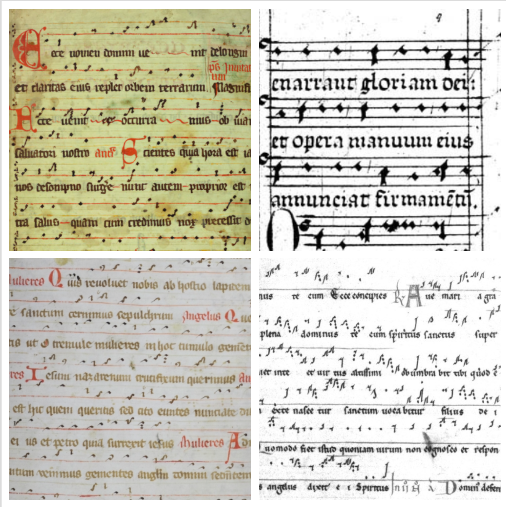
\includegraphics{chant_manuscripts}
\caption{An example of chants as inscribed in manuscripts.}
\label{fig:chant_manuscripts}
\end{figure}

Gregorian chant is a widely researched topic of study, partly thanks to the substantial amount of available sources. However, traditional
musicology is limited by the individual capacity; it is infeasible to study extremely large numbers of chants by hand. This is where
Digital Humanities come into play. Digitalization of large corpora of Gregorian chant enables researchers to draw conclusions
supported by much more data than a human could ever examine.

Nevertheless, contemporary Gregorian chant research still lacks software tools that would facilitate the study of chant repertoire. An example
of an important problem is chant's historical and geographical development. Throughout the 
centuries, the tradition spread accross Europe, while always changing a small part of it. This has led to many variations of the same
chants existing at the same time. Knowing how exactly the changes came into place could shed light on many open questions in the history of 
European culture.

\textbf{The aim of this thesis is to create a tool that musicologists could use to answer questions about chant origin and evolution.} We do this by employing
well-known algorithms for multiple sequence alignment from bioinformatics. Once the idea is proposed, it is almost immediately obvious that
biological and musical sequences share features which warrant using the same methods on both. As opposed to other sequence comparison techniques, such as edit
distance, MSA algorithms do not need any assumptions about the length of chants or other characteristics, which is why they are suitable
for the study of chant.

% screenshot alignmentu s conservation profilom

The tool provides the ability to align a set of chants that is potentially large and diverse in multiple ways, each of which has slightly different uses. One important
implication of the tool is that it makes the discovery contrafacta (chants with the same melody but different lyrics) and transpositions
(chants with the same melody but shifted by an interval) across large repertoires easy.

It is important to note that the purpose of this thesis is not to conduct experiments. It is merely a tool for musicologists who possess
the knowledge needed to select the appropriate data so that previously infeasible discoveries can be made.


\chapter{Related work}

With the advent of computers, the field of Music Information Retrieval (MIR) emerged. Research in this interdisciplinary field focuses on extracting
information from musical notation using computer science methods, such as signal processing or machine learning. Its applications
vary widely, from recommender systems, to automatic audio transcription, to music generation. MIR encompasses all different kinds of music,
regardless of their location, age, or function. Researchers have developed a multitude of software tools that facilitate music analysis,
irrespective of what type of music it is. One of such toolkits is \emph{music21} \citep{music21}, a Python package able to encode musical notation
as Python objects and perform analysis on large datasets.

The study of plainchant using computational methods has not been done extensively. The main research tool for musicologists in this field
is the Cantus Index \citep{cantus_index}. It is an online index of chants from several different chant databases, providing researchers with 
a common API for all of them. The entries in Cantus Index only contain four data fields: full-text, genre, feast (not required), and Cantus ID,
which is automatically assigned to newly added chants. The tool is also able to search for melodies in the original source and even provides 
search-by-melody functionality. There are ten databases indexed in the catalogue, the largest of which is the Cantus database \citep{cantus_db}.

\cite{chant21} developed \emph{chant21}, a Python package able to convert two standard melodic notations, \emph{volpiano} and \emph{gabc} to
a \emph{music21} object, therefore making it easier to study Gregorian chant computationally. The data they used were 
scraped from Cantus database \citep{cantus_db} and GregoBase \citep{gregobase} and released as CantusCorpus and GregoBaseCorpus, respectively.
Finally, they performed two case studies using the package. In the first one, they confirmed the melodic arch hypothesis \citep{melodic_arch}, 
which had previously only been studied manually. Second, they analyzed the relation between differentiæ and antiphon openings \citep{differentiae}
and found that it differs accross modes.

Some of the computational research into plainchant has been centered on mode classification. \cite{mode_huron} used pitch class profiles to
classify modes. They created a pitch-class distribution for each of the eight modes, and used these classes to classify previously unseen data.
\cite{mode_cornelissen} compared three approaches to mode classification: classical approach, which classifies chants based on
the final pitch, range, and the initial pitch; profile approach, which was largely inspired by \cite{mode_huron}; and distributional approach,
which focuses on the melodic aspect of mode. The authors chose various segmentations and representations of chants and used a tf-idf vector
model to classify mode. The study found that we can accurately classify mode even when we discard all absolute pitch information, the melody
contour contains enough information on its own.

A considerable amount of research has been done into the evaluation of melodic similarity, albeit not for Gregorian chant specifically.
\cite{melodic_similarity} provides an overview of the methods. He mentions edit distance, Markov chains, and geometric measurements as
the most widely used ones. \cite{similarity_plot} used an adapted edit distance metric to calculate the similarity of two melodic sequences
by first calculating the similarity for all segments of each of the sequences and then scaling them by a weight function depending on the
segment length, which yielded them what they call a multi-scale similarity stack. The overall similarity was obtained by averaging its values.
Then they used the MSS stack to create a visualization that takes on the shape of a trapezoid that shows which segments of two sequences
are the most similar.

\cite{similarity_bioinf} argue that methods originally developed for bioinformatics have a great potential to be applied to music. They offer
analogies for bioinformatics concepts found in musicology. For example, they liken DNA and proteins to melodic sequences, homologues (proteins that
have the same ancestor) to song covers, evolution to oral transmission, etc. They claim that despite the similarities, MRI has not leveraged the
full potential of bioinformatics methods. In their article, they focus on modelling melodic similarity using multiple-sequence alignment (MSA)
algorithms, therefore not relying on heuristics, as opposed to previous works. Their results revealed that the MAFFT algorithm yields the best
alignemnt, which can be attributed to the algorithm using gap-free segments as anchor points, therefore partitioning melodies into more meaningful
segments than other algorithms.

The general algorithm for calculating pairwise sequence alignment is the Needleman-Wunsch algorithm \citep{needleman}. It uses dynamic programming
to break down the problem into smaller problems. Given two sequences, it starts aligning them from the beginning. At each point, the algorithm checks
whether the two sequences match in the current position, and if not, whether it will leave the elements mismatched or insert a space. In essence,
all possible alignments are computed and scored and the best one is chosen. The algorithm always yields an optimal alignment, therefore it is
used when the quality of the alignment is important. However, because of its time complexity, it is unsuitable for many applications.

Unlike pairwise sequence alignment, multiple sequence alignment has been shown to be NP-complete \citep{msa_complexity}. As such, there is no practical
way of computing an optimal MSA and we must instead rely on heuristics to obtain a sufficiently good alignment.

\cite{msa_overview} provides an overview of modern multiple sequence alignment algorithms. According to him, the most frequently used algorithms use
the progressive approach, where a guide tree is estimated from unaligned sequences and then pairwise alignment algorithms are used to find
the MSA following the tree. He notes that the scoring methods of the pairwise algorithm are essential. There are two main groups of scoring methods:
matrix-based algorithms, where a substitution matrix is used to determine the cost of replacing one symbol with another, and the consistency-based
methods, which use a collection of global and local alignments to calculate a position-specific substitution matrix. The author claims that
the best methods yield indistinguishable results, except for remote homologs with less than 25\% identity.

T-Coffee \citep{t_coffee} uses the progressive approach described above. It was the first algorithm that used a preprocessed collection of 
alignments to create a library that helps create the guide tree. The library is generated using both global and local pairwise alignments.
Thanks to this approach, T-Coffee minimizes the errors made in the first stages of building the MSA, which is a shortcoming of many previous
algorithms, as these errors tend to persist. They combined precomputed local and global alignments and create a function that assigns a weight to
each pairwise alignment depending on how consistent the pair of residues is with the residue pairs from all other alignments. This process
leads to a significant improvement of the results.

MAFFT \citep{mafft} further improves on other methods by using Fast Fourier transform to identify homologues fast. In addition, the authors
propose a simplified scoring system that reduces CPU time while maintaining its accuracy. The authors' results showed a performance 
100 times better than that of T-Coffee. 

Despite the fact that MSA algorithms have already been used for music analysis, this is the first work that focuses specifically on applying
the methods on Gregorian chant. Gregorian chant is specific by its monophonic nature, which means that there is just one sequence to analyze.
Each chant has also undergone many changes over the centuries, therefore there are many variants of the same chants that can be
researched. These characteristics make Gregorian chant an ideal subject for MSA analysis and subsequent application of related bioinformatics methods.

% one sequence to analyze (as is the case of modern repertoire)

\chapter{Data}

Our main source of data is the Cantus database (\cite{cantus_db}), one of the databases indexed in the Cantus Index. The database serves as a 
digital archive of chants, each entry containing information about its source, liturgical occasion, mode, and others. Work on the project started
in the late 1980s, and to date, around 500,000 individual chants from approximately 150 manuscripts have been indexed. Each entry is transcribed 
manually and undergoes a thorough examination before publishing (\cite{cantus_lacoste}).

We are using a scraped version of the Cantus database released as CantusCorpus (\cite(chant21)). Unlike the Cantus database which is continuously being
updated and is therefore unsuitable for computational study, the corpus is versioned, therefore each version always contains the same data. We are using
version 0.2 released in July 2020 which contains 497071 entries. The corpus is available for download in CSV format.

\section{CSV}

CSV is one of the most common formats for tabular data. The abbreviation stands for \emph{comma-separated values}. As the name suggests, the format
uses commas to separate columns (although other separators, such as a semicolon, can be used as well to allow for simpler parsing in case that the data 
frequently contains commas that would otherwise need to be escaped), while the individual rows are separated by a line break. The data is stored as plaintext,
which makes it easily readable. Parsing CSV files becomes more complicated when the data contains column and row separators inside fields; in that case
quotation marks or esape sign has to be used. There exist many well-designed parsers, one such parser is the Python module simply called \emph{CSV}.

\section{Database fields}

The csv files in Cantus Corpus contain 21 fields (excluding its row number), of which we are only using a subset.

Each entry contains the chant's incipit, which is the first few words of the text. As chants do not have a title, incipit can substitute its role
in contexts where one is needed.

The fields position, sequence, and folio represent the exact location of the original chant in a manuscript from which it was transcribed.

feastid represents the liturgical occasion when the chant was intended to be performed, or, in other words, a feast. Similarly, officeid represents
the liturgical time of the day during which it was sung.

The text and melody of the chant are found in the fulltext and volpiano fields, respectively. Entries can contain both, either, or none of these fields.

\section{Volpiano}

The melodies in the volpiano fields are encoded as strings of alphanumeric characters and dashes. These can be rendered as musical notation using
the volpiano font. Each character represents either a pitch, empty space, or other musical characters, such as a clef.

Volpiano was developed as a research tool optimized for databases and word processors. There are strict rules concerning the transcription, which leads
to all volpiano-encoded melodies having a standardized format. Each transcription begins with a treble clef. Gaps between words are encoded as three
dashes, while two dashes represent gaps between syllables (\cite{volpiano}).


\chapter{Multiple sequence alignment}

Sequence alignment, in general, is a task whose purpose is to arrange two or more sequences with a common alphabet to identify similar
and different regions within them. A set of sequences being \emph{aligned} in this case can be understood as each being extended by spaces
in such a way that if they are arranged in a matrix, each sequence occupying one row and each column containing one character, it can be seen
what had to happen for one sequence to change into another on a character-by-character basis: insertion (or deletion), character substitution,
or nothing if the characters in the given position are identical. A good sequence alignment algorithm is one that does not perform
unnecessary insertions (deletions) or substitutions.

The problem of multiple sequence alignment is most studied in bioinformatics. Since DNA was first sequenced
in the 1970s, there has been a need to compare various genomes to determine similarity. As organisms mutate and evolve, their
DNA or RNA changes. Aligning their genomes reveals similar and different regions, which facilitates the tracking of these
mutations and makes it possible to determine the order in which they happened.

However, the applications of sequence alignment are not limited to biology. Every task that makes use of determinig the similarity
of some sequences, where the emphasis is put on finding regions where they do not diverge, can make use of the existing methods.

Melody alignment of Gregorian chant can be considered as such. As the tradition spread across Europe, each place changed some of 
the existing melodies by a little, thereby creating new melodies that can change further as they travel through time and space.
This is akin to the mutations in DNA caused by environmental factors. Finding well-conserved regions in many instances of chant
provides great insight into which parts of a melody are unlikely to change, and, on the other hand, which ones tend to vary
a lot. It can also reveal the ancestors of a melody and the path which it traveled to transform into its final form.
This is in line with the focus of philology shifting not to merely reconstructing an earliest layer of a text (with the unspoken 
assumption that this is the ``real'' text), but to map the entire tradition of text transmission and evolution, taking the later layers 
to be as valid within their cultural environment as the older layers.


In this chapter, we will first give the definition of the problem of sequence alignment. We will mention some important considerations,
as well as theoretical limitations. Then we will provide an overview of the methods developed for bioinformatics that attempt to solve
the problem. Finally, we will show how we applied the existing methods and technologies on Gregorian chant melodies.

\section{The problem of sequence alignment}

Assume that we have an alphabet $\mathcal{A}$ and a character $\sigma$ such that $\sigma \notin \mathcal{A}$. Then let us have a set
of sequences $S = \{s_1, s_2, ..., s_k\}$ with $s_i \in \mathcal{A}^{l_i}$. The output of a sequence alignment algorithm is the set of
aligned sequences $A = \{a_1, a_2, ..., a_k\}$, where $a_k \in (\mathcal{A}\cup\{\sigma\})^L$, $L \geq l_i \:\forall i\in\{1, 2, ..., k\}$.
Each original sequence $s_i$ can be obtained from the aligned sequence $a_i$ by removing all $\sigma$.

Given two aligned sequences $a_i$ and $a_j$ and an index $p \leq L$, we define the following operations:

\begin{itemize}
    \item \emph{Identity}: $(a_i)_k = (a_j)_k$
    \item \emph{Insertion}: $(a_i)_k = \sigma \land (a_j)_k \in \mathcal{A}$
    \item \emph{Deletion}: $(a_i)_k \in \mathcal{A} \land (a_j)_k = \sigma$
    \item \emph{Substitution}: $(a_i)_k \in \mathcal{A} \land (a_j)_k \in \mathcal{A} \land (a_i)_k \neq (a_j)_k$
\end{itemize}

Each of the operations has an associated cost. The cost of substitution can further vary depending on which characters are being
substituted. We can then define the overall cost of the alignment $A$ in different ways, e.g. as the sum of costs over all triples
$(i, j, p) \: \forall i, j \in \{1, 2, ..., k\} \: \forall p \leq L$ or as the sum of costs for unordered pairs $\{i, j\}$ and indices $p$,
in which case insertion and deletion are considered the same operation. The goal of a sequence alignment algorithm is to minimize the cost.
There are other, more complicated ways of defining the cost  function, and the performance of an algorithm is highly dependent on which one it uses.

\subsection{Pairwise and multiple sequence alignment}

Depending on the number of sequences to align, we distinguish between pairwise alignment for pairs of sequences and multiple sequence alignment
for more than two. Despite the similarity in their outcomes, the two problems are fundamentally different from a computational perspective.

Pairwise alignment is relatively easy to solve. The Needleman-Wunsch algorithm, which is a dynamic programming algorithm, can find an optimal
solution in the asymptotic time of $\mathcal{O}(mn)$, where $m$ and $n$ are the respective lengths of the sequences. This means that it is
possible to find an optimal alignment even for longer sequences.

Needleman-Wunsch algorithm can be extended to more than two sequences. However, with each additional sequence, its complexity increases,
and it quickly becomes impractical or even practically impossible to align multiple sequences this way. In fact, it has been proven that multiple sequence
alignment is an NP-complete problem \citep{msa_complexity}. It is therefore necessary to use various heuristics to generate alignments. Current
algorithms do not aim at finding the optimal alignment; instead, they try to produce one that is good enough.

\subsection{Local and global sequence alignment}

There is a distinction to be made between local and global sequence alignment.

The problem description above is the definition of global alignment. Aligning sequences globally means aligning the entire sequences end-to-end.
(This does not mean, however, that there cannot be gaps at the beginning or at the end of the generated alignment.)
All characters from all sequences must be present in the final alignment. Global alignment is used to compare relatively similar
sequences, such as protein homologues or versions of the same chant sung at different points in time.

On the other hand, the goal of local alignment is to find similar regions in divergent sequences, while the rest of the sequences is disregarded.
The output of local alignment algorithms contains only a substring of both sequences. Local alignment is suitable for finding conserved patterns.

Both methods are useful in their own way. Local alignment provides a slightly different insight than global alignment, however, they can
be combined to extract more information. In fact, the best current multiple sequence alignment algorithms use local alignment for pairs
of sequences to generate a better overall global alignment. \citep{msa_overview}

\section{Sequence alignment methods}

The methods used to find sequence alignments depend on how many sequences there are and whether they should be aligned globally or locally.
Dynamic programming can used for finding pairwise alignment, both local and global. For many sequences, other methods have been developed. They
do not compute the optimal alignment, however, by using appropriate heuristics, their output is good enough.

\subsection{Pairwise alignment: dynamic programming}

Dynamic programming techniques are useful for pairwise alignment. The Needleman-Wunsch algorithm \citep{needleman} computes the global alignment
of two sequences. A variation of the algorithm, the Smith-Waterman algorithm \citep{smith_waterman}, computes the local alignment of two sequences.

\subsubsection{Needleman-Wunsch algorithm}

The idea of the algorithm is to start with two empty sequences and subsequently add characters from either or both of the given sequences so as
to obtain an optimal alignment in each step. Namely, suppose that we have two sequence prefixes $A$ and $B$ that have already been aligned optimally
and their alignment gives a score of $s$. Furthermore, suppose that the next characters in the sequences are $a$ and $b$, respectively. There are
three possibilities:

\begin{itemize}
    \item We append $a$ and $b$ to the respective prefixes. By doing so, we obtain the aligned sequence prefixes $Aa$ and $Bb$.
        \begin{verbatim}
            Aa
            Bb
        \end{verbatim}
    \item We append $a$ to $A$ and a gap to $B$. This way, we get the aligned prefixes $Aa$ and $B$.
        \begin{verbatim}
            Aa
            B-
        \end{verbatim}
    \item We append a gap to $A$ and $b$ to $B$. Now we have aligned the prefixes $A$ and $Bb$.
        \begin{verbatim}
            A-
            Bb
        \end{verbatim}
\end{itemize}

Each of the possibilities adds a value to the score $s$ depending on what characters were added. To get the optimal alignment, we choose the one
that yields the highest score. We then proceed to the next character, having two optimally aligned prefixes $A'$ and $B'$. This leads to a recursive
algorithm that can be formulated using dynamic programming.

Let us have two input sequences, $A$ and $B$ of lengths $m$ and $n$ with a common alphabet $\mathcal{A}$ and the gap character $\sigma$.
Let us define the scoring function $s$ as

\[ s(a, b) = 
    \begin{cases}
        1  & \text{if } a = b \\
        -1 & \text{if } a = \sigma \lor b = \sigma \\
        -1 & \text{if }  a \neq b
    \end{cases}
\]

The algorithm initializes a matrix $M$ of size $(m+1) * (n+1)$. The rows and columns represent the characters of $A$ and $B$, respectively, except
for the first row and the first column, which represent the beginning of a sequence or an empty sequence. That is to say, the row $M_{i, *}$ represents the
character $A_{i-1}$ for $i \geq 2$ and analogically, the column $M_{*, j}$ represents the character $B_{j-1}$ for $j \geq 2$.

The algorithm iterates over the rows and columns of the matrix. In each step, it calculates the value of a cell $M_{i,j}$, provided that each of the cells $M_{i-1, j}$,
$M_{i, j-1}$ and $M_{i-1, j-1}$ have been filled out, as

\[ M_{i, j} = max
    \begin{cases}
        M_{i-1, j-1} + s(A_{i-1}, B_{j-1}) \\
        M_{i-1, j} + s(A_{i-1}, \sigma)    \\
        M_{i, j-1} + s(\sigma, B_{j-1})
    \end{cases}
\]

In other words, the algorithm either aligns the two characters in positions $i-1$ and $j-1$, or it inserts a gap into sequence $B$, or it inserts a gap into sequence $A$,
and chooses the version which yields the highest score.

The first row and column are apparently special cases, as there is no previous row or column. Therefore, for each cell in the first row or column, there is
only one possible choice of score, which is equivalent to inserting a space.

After filling out the entire matrix, the algorithm then finds the optimal alignment by backtracking in the matrix. It starts in the bottom right
cell of the matrix, which represents both sequences being aligned. In each iteration, it looks at the cells above, to the left and to the top-left
of the current positions and chooses the highest score. If it moves top or left, it means that a gap was inserted. Moving diagonally represents a match
or mismatch. By tracing its way back to the top left corner, the algorithm finds the alignment that yielded the highest score.

Let us show the algorithm on an example. Consider two sequences of nucleotide residues:

\begin{verbatim}
    GATTA
    GCATG
\end{verbatim}

The matrix is initialized without anything filled out.

% create a figure

\begin{verbatim}
          G  C  A  T  G
      
    G 
    A 
    T 
    T 
    A 
\end{verbatim}

We start filling out the matrix in the top left corner. Using the basic scoring scheme (+1 for a match, -1 for everything else), we insert a 0
to the beginning, and, since there is no top cell for the first row and no left cell for the first column, we add -1 to each subsequent cell,
representing a gap insertion.

\begin{verbatim}
          G  C  A  T  G
       0 -1 -2 -3 -4 -5
    G -1
    A -2
    T -3
    T -4
    A -5
\end{verbatim}

The next cell to fill out is the one in the first \verb|G| column and the first \verb|G| row. We have three options:

\begin{itemize}
    \item Move from the top, represents gap insertion for a score of -1. The final score would be $(-1) + (-1) = -2$.
    \item Move diagonally, represents match, giving a score of +1. The score in this case would be $0 + 1 = 1$.
    \item Move from the left, i.e. gap insertion. The score would be $-2$ as in the first case.
\end{itemize}

We choose the highest score, which in this case is a diagonal move representing a match. It follows intuition: we are now aligning
\verb|G| and \verb|G|, matching them seems logical.

\begin{verbatim}
          G  C  A  T  G
       0 -1 -2 -3 -4 -5
    G -1  1
    A -2
    T -3
    T -4
    A -5
\end{verbatim}

Now let us look at the cell in the \verb|C| column and the \verb|G| row. Moving from the top yields -3, moving from the left yields
0 and moving diagonally yields -2, as it is a mismatch in this case. The highest of these scores is 0.

\begin{verbatim}
          G  C  A  T  G
       0 -1 -2 -3 -4 -5
    G -1  1  0
    A -2
    T -3
    T -4
    A -5
\end{verbatim}

We continue filling out the table this way until it is complete.

\begin{verbatim}
          G  C  A  T  G
       0 -1 -2 -3 -4 -5
    G -1  1  0 -1 -2 -3
    A -2  0  0  1  0 -1
    T -3 -1 -1  0  2  1
    T -4 -2 -2 -1  1  1
    A -5 -3 -3 -1  0  0
\end{verbatim}

As we have now calculated the scores for all prefixes, we can use backtracking to find the optimal alignment for the two sequences.
Starting in the bottom right cell, we choose the cell (top, left or top-left) with the highest score. If multiple cells have the same score, we can 
choose either. The different alignments the cells represent are all optimal. The cell that we choose gives us the optimal alignment
of the sequences before the last character was added. Depending on the direction by which we moved, we know whether this last character
was a character of the sequence or a gap.

For example, consider the bottom right corner of the matrix.

\begin{verbatim}
       T  G
    T  1  1
    A  0  0
\end{verbatim}

Starting in the bottom right, we can choose either the top or the top-left cell. Choosing the top-left one, i.e. moving diagonally, means that
the last characters in the alignment were \verb|A| and \verb|G| for the respective sequences. We can find the alignment of the prefixes \verb|GATT|
and \verb|GCAT| by backtracking from the top-left cell. By contrast, choosing the top cell means inserting a gap in the second sequence, and by backtracking
from there we can find the alignment of \verb|GATT| and \verb|GCATG|.

\begin{figure}[h]
    \begin{equation*}
        \begin{matrix}
                &            & G          & C          & A          & T          & G        \\
                & \rn{00}{0} & -1         & -2         & -3         & -4         & -5       \\
            G   & -1         & \rn{11}{1} & 0          & -1         & -2         & -3       \\
            A   & -2         & 0          & \rn{22}{0} & \rn{23}{1} & 0          & -1       \\
            T   & -3         & -1         & -1         & 0          & \rn{34}{2} & 1        \\
            T   & -4         & -2         & -2         & -1         & \rn{44}{1} & 1        \\
            A   & -5         & -3         & 3          & -1         & 0          & \rn{55}{0}
        \end{matrix}
    \end{equation*}

    \begin{tikzpicture}[overlay,remember picture]
        \draw [->] (55) -- (44);
        \draw [->] (44) -- (34);
        \draw [->] (34) -- (23);
        \draw [->] (23) -- (22);
        \draw [->] (22) -- (11);
        \draw [->] (11) -- (00);
    \end{tikzpicture}
\caption{A path representing an optimal alignment.}
\label{alignment_path}
\end{figure}


Figure \ref{alignment_path} shows a path that represents the alignment

\begin{verbatim}
    G A - T T A
    G C A T - G
\end{verbatim}

\subsubsection{Smith-Waterman algorithm}

The algorithm is similar to Needleman-Wunsch algorithm. As its purpose is to find an optimal local alignment, it does not
penalize long regions of mismatches or gaps. Its purpose is to find regions with the most matches. The only difference from the Needle\-man-Wunsch 
algorithm is in how new matrix cells are filled out. Namely, when willing out a new cell, we use the formula

\[ M_{i, j} = max
    \begin{cases}
        0   \\
        M_{i-1, j-1} + s(A_{i-1}, B_{j-1}) \\
        M_{i-1, j} + s(A_{i-1}, \sigma)    \\
        M_{i, j-1} + s(\sigma, B_{j-1})
    \end{cases}
\]

In other words, all negative values in what would be the matrix from Needle\-man-Wunsch algorithm are replaced by 0.

\subsection{Multiple sequence alignment: progressive methods}

As has already been mentioned, it is essentially impossible to use dynamic programming to compute the alignment of more than two sequences.
Therefore, other methods have been developed. The most successful ones appear to be the so-called progressive methods. In general,
they use some heuristics to estimate a guide tree, which is a phylogenetic tree determining how close the sequences are to each other,
and then they compute the actual multiple alignment following the order of this tree.

One of such methods is the Tree-based Consistency Objective Function for alignment Evaluation (T-Coffee) algorithm \citep{t_coffee}.
Its most important contribution is its extended library generated from both local and global pairwise alignments of all pairs of input sequences.
This library enables the algorithm to make fewer mistakes in the initial stages of the guide tree, as these errors propagate throughout the entire tree.

\begin{figure}[h]
\centering
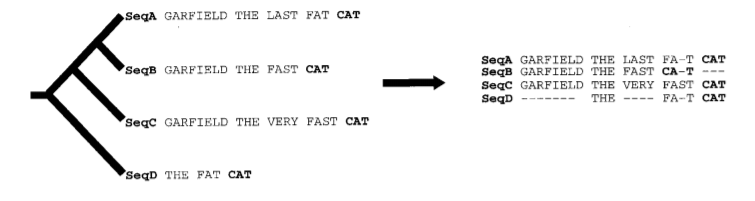
\includegraphics[scale=0.85]{t-coffee-errors}
\caption{Misalignment of the word CAT using other progressive methods. \citep[Figure~2(a)]{t_coffee}}
\end{figure}

Another method is MAFFT (the name presumably coming from the acronyms for multiple alignment and fast Fourier transform) \citep{mafft}.
The authors focused on finding alignments that are not only optimal, but also biologically correct. They developed a way of rapid identification
of homologous regions between two sequences using FFT, and then used the better pairwise alignments to create a better multiple alignment.

\subsubsection{T-Coffee}

The T-Coffee algorithm consists of various stages. The first one is to compute pairwise alignments for all pairs of input sequences.
Two primary libraries are generated, one for global and one for local alignments. Each can contain more than one alignment for each pair.

As some alignments tend to be more correct than others, weighting is then performed. The authors chose sequence identity of two aligned
sequences as the weight of each of the aligned residues in the pair. For example, consider the sequences $A$ \verb|GARFIELD THE LAST FAT CAT|
and $B$ \verb|GARFIELD THE FAST CAT|. If they are aligned as

\begin{verbatim}
    GARFIELD THE LAST FAT CAT
    GARFIELD THE FAST CAT ---
\end{verbatim}

then their sequence identity is 88\%, as there are two non-equal characters aligned (i.e. there is no gap penalty). Therefore, the weight of
each residue pair $W(A(x), B(y))$, where $A(x)$ denotes the character $x$ from sequence $A$, and analogically for $B(y)$, is equal to 88.

\begin{figure}[h]
\centering
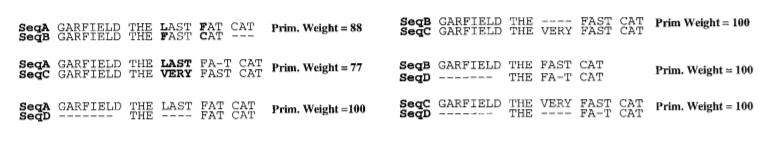
\includegraphics[scale=0.85]{t-coffee-primary-lib}
\caption{Primary library created from 4 sequences. \citep[Figure~2(b)]{t_coffee}}
\end{figure}

The two primary libraries are then combined into one by combining all identical residue pairs into one entry and summing their weights, while
pairs that are only present once are added with their original weight. Residue pairs that are not present in any alignment have an implicit weight
of 0.

Although the information present in the primary library is sufficient to obtain a multiple alignment, it is computationally hard to do so. Instead,
the authors chose to generate what they call an extended library using the weights in the primary library.

Library extension is performed by comparing each aligned residue pair with all the others. Consider a residue pair $(A(x), B(y))$ and a sequence $C$.
The initial weight of the pair is then increased by $min(W(A(x), C(z)), W(C(z), B(y)))$, i.e. the minimum weight associated to the alignment of some
residue $C(z)$ with both $A(x)$ and $B(y)$. This is done for all residues from all sequences. In practice, most of the weights will be 0, therefore 
the actual algorithm computes the weights more efficiently. Library extension in effect computes how consistent a residue-pair alignment is.

\begin{figure}[h]
\centering
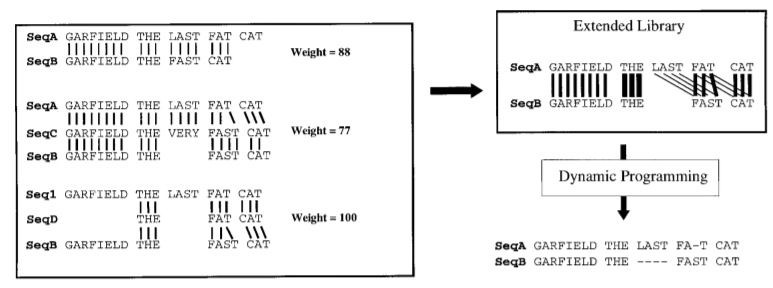
\includegraphics[scale=0.85]{t-coffee-extended-lib}
\caption{Extended library weights for two sequences and their alignment recomputed using these weights. \citep[Figure~2(c)]{t_coffee}}
\end{figure}

Having obtained the consistency information from the extended library, it is now possible to create the guide tree and the final multiple alignment.
Using a distance matrix between all the sequences, the tree is computed as follows. First, we align the closest two sequences using dynamic programming
and the weights from the extended library. In each of the following steps, we either add a sequence to an already computed alignment, or we align
the next closest sequences. We repeat this step until the alignment of all sequences is complete.

\begin{figure}[h]
\centering
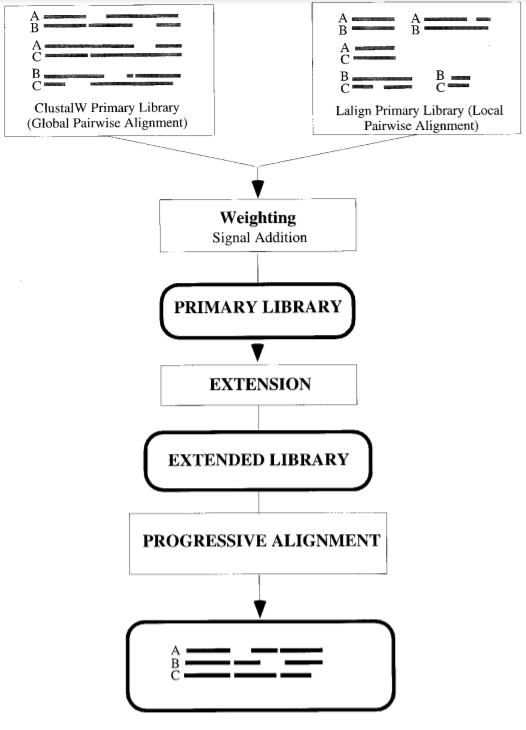
\includegraphics[scale=0.5]{t-coffee-flowchart}
\caption{T-Coffee layout. \citep[Figure~1]{t_coffee}}
\end{figure}

\subsubsection{MAFFT}

The MAFFT method is similar to T-Coffee in that it constructs a library of alignments which it then uses to create the final multiple alignment. The authors developed MAFFT
to work in multiple modes, one of which is the progressive method as described above; the other one is the iterative refinement method, which allows for alterations
of the multiple alignment obtained from the progressive method.

Pairwise alignment in MAFFT uses the fact that certain amino acids have more similar physico-chemical properties than others. Substitutions tend to preserve the
overall structrure of a protein, therefore substitutions of similar amino acids are more frequent than those of different ones. The two properties
the authors use are amino acid volume and polarity.

Let us define the correlation of the volume component between two amino acid sequences with the positional lag of $k$ as

\[
    c_v(k) = \sum_{1\leq n \leq N, 1 \leq n+k \leq M} \hat{v}_1(n) \hat{v}_2(n+k)
\]
where $N$ and $M$ are the lengths of the sequences and $\hat{v}(a) = [v(a) - \bar{v}] / \sigma_v$ is the normalized volume value with $\bar{v}$
denoting the average volume of all the amino acids and $\sigma_v$ their standard deviation.

Since the sequences tend to be equal in length, computing $c_v(k)$ using naive methods takes time proportional to $N^2$. However, applying Fast Fourier
transform to the calculation reduces the time to $\mathcal{O}(N log N)$.

We define the polarity component correlation $c_p(k)$ analogically.

The correlation between two amino acids is then expressed as 

\[
    c(k) = c_v(k) + c_p(k)
\]

\begin{figure}[h]
\centering
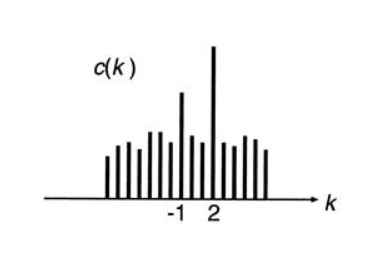
\includegraphics{mafft_correlation_plot}
\caption{Plot of the correlation function $c(k)$. \citep[Figure~1A]{mafft}}
\label{fig:mafft1}
\end{figure}

If we plot the function $c(k)$, there will be some peaks corresponding to the homologous regions of the two sequences, if there are any (Figure \ref{fig:mafft1}). However, the FFT
analysis only gives us the positional lag of the regions, not their positions. To find the exact positions, we use a sliding window (of size 30 in the article)
and calculate the degree of local homologies for the 20 highest peaks in the $c(k)$ function. If a segment exceeding a given homology threshold is identified,
we label it as a homologous region.

\begin{figure}[h]
\centering
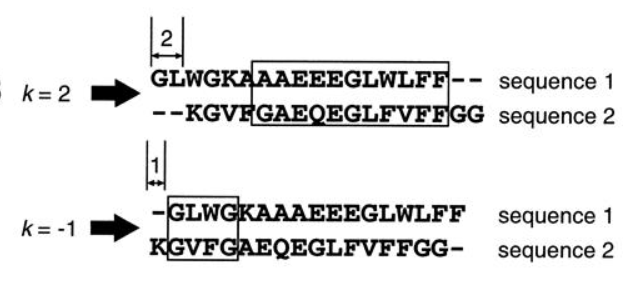
\includegraphics{mafft_sliding_window}
\caption{Finding homologous regions with different positional lags using a sliding window. \citep[Figure~1B]{mafft}}
\label{fig:mafft2}
\end{figure}

After finding homologous segments between two sequences, their alignment is obtained by constructing a homology matrix $S \in R^{n*n}$, where $n$ is the number of homologous
segments. The cell $S_{ij}$ is assigned a value depending on whether the $i$-th homologous segments of the first sequence corresponds to the $j$-th homologous segment
of the second sequence. If so, the cell gets a value corresponding to the score of this segment; otherwise it has a value of 0. The optimal arrangment of homologous segments
is then obtained using dynamic programming.

\begin{figure}[h]
\centering
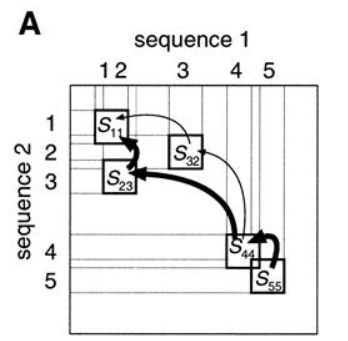
\includegraphics{mafft_optimal_path}
\caption{Dynamic programming applied on segment arrangement. \citep[Figure~2A]{mafft}}
\label{fig:mafft3}
\end{figure}

Having arranged homologous segments, the algorithm then computes pairwise alignments for each pair of sequences. As in T-Coffee, it uses the alignments to create
the primary and extended libraries, which are in turn used to estimate the guide tree and the final alignment. If MAFFT is configured to perform the progressive 
method, this alignment is the final one. Otherwise, if iterative refinement is allowed, MAFFT uses the weights from the library to adjust the alignment to get a more
optimal one. However, iterative refinement is very slow from a relatively low number of sequences, therefore it is not suitable for a large dataset.

\section{Sequence alignment for chant melodies}

As we have discussed before, melodies of Gregorian chant are in many ways similar to biological sequences. The alphabet is different (instead of 20 amino acids
in proteins or 4 nucleotide bases in DNA we have around 40 different characters used in melody representation) and the chants are usually shorter in length.
The evolution of both biological and melodic sequences is guided by environmental factors such as migration to other places. Some segments tend to undergo a lot
of modifications, while other remain relatively unchanged. Studying the alignment of chant melodies can reveal a lot of information about their relationship.

In the following sections, we describe three approaches to melody alignment used in our application.

The first one is a naive approach. It merely aligns all chants to have the same number of words and each word to have the same number of syllables, filling the extra
positions with gaps, if needed.

The other two approaches use MAFFT to perform a proper sequence alignment. They differ in what we are aligning. One of them aligns notes and other symbols as they are;
each representing a certain pitch. The other one is more sophisticated: it does not use the absolute value of the pitches, but rather the intervals between the notes.
This way, we can see segments that have merely been shifted by a certain interval.

\subsection{Naive alignment}

\subsection{Multiple alignment using absolute pitches}

For this task, we are using the MAFFT software\footnote{https://mafft.cbrc.jp/alignment/software/}. As the software uses the character \verb|-| for marking gaps,
it requires that the input sequences do not contain any, or they will be removed. Since melodies encoded as Volpiano use the character to mark ends of words
and ends of syllables, we need to perform some preprocessing. Namely, we replace all contiguous sequences \verb|---| with the end-of-word marking symbol \verb|~|
and all contiguous sequences \verb|--| with the end-of-syllable marker \verb=|=. All remaining \verb|-|s are removed, if there are any.

The sequences are then passed to MAFFT with the option \verb|--text|, which indicates that the sequences are not biological. Additionally, we also pass the option
\verb|--reorder|, which returns the aligned sequences in order of similarity. We made this choice so as to facilitate the identification of related melodies.

After MAFFT performs the alignment, we retrieve the sequences and attempt to combine them with their text.
We do this by splitting both the text and the melody into syllables and mapping them onto each other (Algorithm \ref{algo:volpiano_text_combine}). 
However, this might not be possible. Due to errors in the original encoded melody (i.e. a missing or an extra \verb|-|),
we may have altered the structure of the chant in preprocessing. In case of such event, we remove the affected sequence from consideration and align the remaining
sequences again.\newline

\begin{algorithm}[H]
\SetKwInOut{Input}{input}\SetKwInOut{Output}{output}
    \Input{\emph{volpiano}: melody divided into words and those into syllables, and \emph{text}: lyric divided analogically}
    \Output{\emph{volpiano} and \emph{text} aligned}
    \BlankLine
    set \emph{aligned\_text\_and\_melody} to be an empty list\;
    \For{word at index i}{
        open new word in \emph{aligned\_text\_and\_melody}\;
        \uIf{i-th word of text has more syllables than i-th word of melody}{
            merge the extra syllables into the last one\;
        }
        \uElseIf{i-th word of text has fewer syllables than i-th word of melody}{
            extend the i-th word of text by empty syllables to match the volpiano word
        }
        \For{syllable at index j of i-th word}{
            combine text and melody of the j-th syllable of the i-th word and add it to the current word\;
        }
        close current word\;
    }
    return \emph{aligned\_text\_and\_melody}\;
    \caption{Aligning melody and lyric}
    \label{algo:volpiano_text_combine}
\end{algorithm}

Once all sequences are successfully aligned without errors in text and melody combination, we can display them to the user. In the application, we use the Volpiano font,
so as to maintain consistency. However, the sequences shown are not properly encoded in Volpiano format. First of all, we choose different representations of end of a word
(here we use a bar line) and end of a syllable (a single space) so that the number of characters in each sequence remains equal and the alignment is visible. Second of all,
after the alignment, MAFFT will have inserted \verb|-|s to represent gaps. In proper Volpiano, these characters represent gaps between words, syllables, and neumes. However,
here they just mean empty space.\newline

\begin{algorithm}[H]
\SetKwInOut{Input}{input}\SetKwInOut{Output}{output}
    \Input{a set of volpiano-encoded melodies with their respective lyrics}
    \Output{aligned melodies combined with their lyrics}
    \BlankLine
    preprocess all melodies to a MAFFT-friendly format\;
    \While{melodies have not been aligned without error}{
        run MAFFT on all melodies\;
        \For{aligned melody}{
            combine melody with its text\;
            \If{melody and text cannot be combined}{
                remove melody from list\;
                remember to run the while loop again\;
            } 
        }
    }
    return list of aligned melodies combined with their texts\;
    \caption{Multiple alignment using absolute pitches}
    \label{algo:align_pitch}
\end{algorithm}

\subsection{Multiple alignment using intervals}

The general outline of the algorithm is the same as Algorithm \ref{algo:align_pitch}. However, as we are not aligning absolute pitches, but rather intervals,
we need to compute these intervals.

There are 18 possible pitches, which means 37 possible intervals (17 positive, 17 negative, and one without the change of pitch). We will represent the no-change interval
with the character \verb|a|, the positive intervals with the lowercase characters \verb|b-t| and the negative intervals with the uppercase characters \verb|B-T|. The characters
\verb|i| and \verb|I| are not used for reasons explained later.

The interval representation is constructed from a Volpiano-encoded melody by replacing the note symbols with the appropriate interval symbol. The $i$-th note will be
replaced with the symbol representing the interval $(i-1, i)$. As the first note has no predecessor, it is left as it is. The non-note symbols also remain unchanged.\newline

\begin{algorithm}[H]
\SetKwInOut{Input}{input}\SetKwInOut{Output}{output}
    \Input{volpiano-encoded melody}
    \Output{interval representation of the input melody}
    \BlankLine
    $interval\_representation \longleftarrow ""$\;
    \For{character c in volpiano}{
        \uIf{c is a non-note character}{
            append c to \emph{interval\_representation}\;
        }
        \uElseIf{c is a note-representing character and it is the first such one}{
            append c to \emph{interval\_representation}\;
            $last\_seen\_note \longleftarrow c$\;
        }
        \uElse{
            $interval \longleftarrow (last\_seen\_note, c)$\;
            $i \longleftarrow symbol \: for \: interval$\;
            append i to \emph{interval\_representation}\;
            $last\_seen\_note \longleftarrow c$\;
        }
    }
    return \emph{interval\_representation}\;
    \caption{Converting volpiano-encoded melody into interval representation}
    \label{algo:convert_to_interval}
\end{algorithm}

We use the interval representations as inputs to MAFFT. That means that what MAFFT returns are the aligned sequences of intervals. To display them to the user
properly, we need to decode the sequences.\newline

\begin{algorithm}[H]
\SetKwInOut{Input}{input}\SetKwInOut{Output}{output}
    \Output{interval representation of a melody}
    \Input{volpiano-encoded equivalent of the input melody}
    \BlankLine
    $volpiano \longleftarrow ""$\;
    \For{character c in interval representation}{
        \uIf{c is a non-interval character}{
            append c to \emph{volpiano}\;
        }
        \uElseIf{c is a note-representing character and it is the first such one}{
            append c to \emph{volpiano}\;
            $last\_seen\_note \longleftarrow c$\;
        }
        \uElseIf{c is an interval-representing character and we have already seen the first note}{
            $note \longleftarrow last\_seen\_note +$ interval represented by $i$\;
            append note to \emph{volpiano}\;
            $last\_seen\_note \longleftarrow note$\;
        }
    }
    return \emph{volpiano}\;
    \caption{Converting interval representation back to volpiano}
    \label{algo:decode_interval}
\end{algorithm}

The reason why we are not using \verb|i| and \verb|I| as symbols for an interval is that as we are looking at whether a character is a note or an interval or neither, 
if they represented an interval, we would choose the appropriate branch in Algorithm \ref{algo:decode_interval}. However, marking an interval is not the only way how
the character could have got there: \verb|i| and \verb|I| represent non-note elements in the Volpiano protocol. Therefore, we could mistakenly shift the melody by an interval,
as there is no way of knowing which case it is.

The complete algorithm is similar to Algorithm \ref{algo:align_pitch}.\newline

\begin{algorithm}[H]
\SetKwInOut{Input}{input}\SetKwInOut{Output}{output}
    \Input{a set of volpiano-encoded melodies with their respective lyrics}
    \Output{aligned melodies combined with their lyrics}
    \BlankLine
    convert all melodies to interval representations\;
    preprocess all interval representations to a MAFFT-friendly format\;
    \While{melodies have not been aligned without error}{
        run MAFFT on all interval representations\;
        \For{aligned interval representation}{
            convert interval representation to volpiano-encoded melody\;
            combine melody with its text\;
            \If{melody and text cannot be combined}{
                remove melody from list\;
                remember to run the while loop again\;
            } 
        }
    }
    return list of aligned melodies combined with their texts\;
    \caption{Multiple alignment using intervals}
    \label{algo:align_intervals}
\end{algorithm}


\chapter*{Conclusion}
\addcontentsline{toc}{chapter}{Conclusion}

The outcome of this thesis is an interdisciplinary software tool applying methods from bioinformatics to digital musicology, enabling researchers
to analyze relatively large amounts of data computationally. The software
provides the ability to investigate the origin and evolution of a set of chants. An important implication of this ability is that it facilitates
the discovery of contrafacta (chants with different lyrics but the same melodies) and transpositions (chants whose melodies differ by an interval
in all positions), which is a task that lacked the proper tools until now.

To analyze the chants, we used techniques from bioinformatics, namely multiple sequence alignment algorithms. These techniques have been used by
biologists for a long time to study the same properties - origin and evolution - of biological sequences. As chant melodies and biological sequences
share many properties, and, importantly, MSA algorithms do not require assumptions about chants that we cannot guarantee, these methods are suitable
for studying Gregorian chant.

Our work bridges the gap between traditional musicology,
which relied on the individual ability to draw conclusions from analog sources, and computational analysis. The software is a tool
that will have immediate applications in the basic research of Gregorian chant, such as the study of \emph{Jistebnice Cantionale}.\footnote{
Done in collaboration with the \emph{Old Myths, new Facts} project at the Masaryk Institute of the Czech Academy of Sciences and the Faculty
of Arts of Charles Univeristy.}

Originally, one of the purposes of this work was to create a set of visualizations that would facilitate the quantitative analysis of a set of chants.
However, during the development process it became clear that musicology itself has not yet formalized many of its problems in such a way that 
would make it clear what types of quantitative analysis is actually needed.\footnote{From personal communication with Dr. Jennifer Bain and Dr.
Debra Lacoste.} In fact, the alignment tool proved to be much more useful for immediate
applications\footnote{From personal communication with doc. PhDr. Hana Vlhová-Wörner, Ph.D}. Therefore, our attention shifted to the proper
development of the alignment tool. The visualization part is left for further development, in hopes that the desired use cases crystallize into
a more definite form in the future.

The software continues to be developed in collaboration with the Czech Aca\-demy of Sciences.

\section*{Future work}

Computing multiple sequence alignment opens the door to many other applications. Our software touches upon one
of them by providing the ability to calculate the conservation profile; thhe natural next step is to use the results of the alignment to
obtain and visualize the phylogenetic tree of the set, i.e. their
``family tree'' showing how the individual melodies changed and developed. The tree's visualization could make it easier to see
the relationship between the melodies without the need to study the alignment.

Another possibility is to use the similarity matrix obtained from the alignment to visualize a network of the chants. The clusters
forming in this visualization could show related groups of chants and reveal relationships that were not obvious before.

The opportunities promised by MSA algorithms are vast. We plan to explore more of those that will be determined to be useful for the study of Gregorian
chant, as we continue with the development of the software in collaboration with chant researchers, and we are looking forward to new discoveries.


%%% Bibliography
%%% Bibliography (literature used as a source)
%%%
%%% We employ bibTeX to construct the bibliography. It processes
%%% citations in the text (e.g., the \cite{...} macro) and looks up
%%% relevant entries in the bibliography.bib file.
%%%
%%% The \bibliographystyle command selects, which style will be used
%%% for references from the text. The argument in curly brackets is
%%% the name of the corresponding style file (*.bst). Both styles
%%% mentioned in this template are included in LaTeX distributions.

\bibliographystyle{plainnat}    %% Author (year)
% \bibliographystyle{unsrt}     %% [number]

\renewcommand{\bibname}{Bibliography}

%%% Generate the bibliography. Beware that if you cited no works,
%%% the empty list will be omitted completely.

\bibliography{bibliography}

%%% If case you prefer to write the bibliography manually (without bibTeX),
%%% you can use the following. Please follow the ISO 690 standard and
%%% citation conventions of your field of research.

% \begin{thebibliography}{99}
%
% \bibitem{lamport94}
%   {\sc Lamport,} Leslie.
%   \emph{\LaTeX: A Document Preparation System}.
%   2nd edition.
%   Massachusetts: Addison Wesley, 1994.
%   ISBN 0-201-52983-1.
%
% \end{thebibliography}


%%% Figures used in the thesis (consider if this is needed)
\listoffigures

%%% Tables used in the thesis (consider if this is needed)
%%% In mathematical theses, it could be better to move the list of tables to the beginning of the thesis.
\listoftables

%%% Abbreviations used in the thesis, if any, including their explanation
%%% In mathematical theses, it could be better to move the list of abbreviations to the beginning of the thesis.
\chapwithtoc{List of Abbreviations}

%%% Attachments to the bachelor thesis, if any. Each attachment must be
%%% referred to at least once from the text of the thesis. Attachments
%%% are numbered.
%%%
%%% The printed version should preferably contain attachments, which can be
%%% read (additional tables and charts, supplementary text, examples of
%%% program output, etc.). The electronic version is more suited for attachments
%%% which will likely be used in an electronic form rather than read (program
%%% source code, data files, interactive charts, etc.). Electronic attachments
%%% should be uploaded to SIS and optionally also included in the thesis on a~CD/DVD.
%%% Allowed file formats are specified in provision of the rector no. 72/2017.
\appendix
\chapter{Attachments}

\section{First Attachment}

\openright
\end{document}
